\documentclass[11pt]{article}

\usepackage[margin=1in]{geometry}
\usepackage{lmodern}
\usepackage[T1]{fontenc}
\usepackage{microtype}
\usepackage{amsmath,amssymb}
\usepackage{graphicx}
\usepackage{booktabs}
\usepackage{xcolor}
\usepackage{caption}
\usepackage{subcaption}
\usepackage{authblk}
\usepackage{tikz}
\usetikzlibrary{arrows.meta,positioning,fit,backgrounds}
\usepackage[colorlinks=true,allcolors=blue!55!black]{hyperref}

\newcommand{\ProbeRMSE}{0.81}
\newcommand{\ForecastStepOne}{0.0006}
\newcommand{\ForecastStepK}{0.036}
\newcommand{\ForecastHorizon}{30}
\newcommand{\AnomalyPeak}{55}
\newcommand{\AnomalyInjected}{24}
\newcommand{\AnomalyDetected}{22}
\newcommand{\EmbStd}{3.0}


\captionsetup{font=small,labelfont=bf}
\setlength{\parskip}{2pt}

\title{\textbf{DVD-JEPA: A Minimal, Reproducible Joint-Embedding\\
Predictive Architecture World Model}}
\author[1]{Mandar Wagh}
\affil[1]{Black Robotics \quad \texttt{roboticsblack@gmail.com}}
\date{June 2026}

\begin{document}
\maketitle

\vspace{-1.2em}
\begin{center}
\small
Code: \href{https://github.com/mandarwagh9/dvd-jepa}{\texttt{github.com/mandarwagh9/dvd-jepa}} \;$\cdot$\;
Interactive demo: \href{https://dvd-jepa.vercel.app}{\texttt{dvd-jepa.vercel.app}}
\end{center}

\begin{abstract}
\noindent
A \emph{world model} predicts how an environment evolves. The dominant failure mode when learning one
from video is generative: predicting future pixels forces the model to spend capacity on detail that is
fundamentally unpredictable. Joint-Embedding Predictive Architectures (JEPA) instead predict the
\emph{representation} of the future and let the encoder discard what it cannot predict. We present
\textbf{DVD-JEPA}, the smallest honest instance of this idea we could construct: a context encoder, an
exponential-moving-average (EMA) target encoder, and a latent predictor are trained---without labels and
without a decoder---to predict the next observation of a bouncing DVD logo in a $32$-dimensional
representation space. Despite never receiving a coordinate, a frozen linear probe recovers the logo's
position to \ProbeRMSE\,px in a $16$\,px box. An ablation shows that removing the stop-gradient collapses
the representation to a constant, while the EMA target prevents it. Adding an optional decoder turns the
model into a future-frame video predictor that tracks the bounce for ${\sim}20$ steps before latent
rollout drift, and into a predictive anomaly detector whose surprise signal spikes \AnomalyPeak$\times$
over baseline on an injected teleport. The entire model trains on a CPU in ${\sim}10$ seconds and the
trained weights run client-side in a browser. DVD-JEPA is deliberately a toy, but every component has a
full-scale counterpart in I-JEPA, V-JEPA, and V-JEPA~2; it is meant as a transparent, runnable artifact
for understanding how JEPA world models work.
\end{abstract}

\section{Introduction}
A world model answers a single question: given the current state and (optionally) an action, what
happens next? Animals build such models from passive observation, and learning them from video is a
central goal of self-supervised representation learning~\cite{lecun2022,ha2018}. The obvious approach is
\emph{generative}---predict the next frame pixel by pixel---but this is the wrong objective. Most of the
future is unpredictable in its fine detail (exact textures, noise) yet entirely predictable in the
abstract (an object keeps moving). A pixel-predicting model is forced to model the irreducible noise and
produces blurry, hedged predictions.

The Joint-Embedding Predictive Architecture (JEPA) makes a different bet~\cite{lecun2022,assran2023}:
predict in representation space, not pixel space, and let the encoder make itself invariant to whatever
it cannot predict. This is the principle behind I-JEPA for images~\cite{assran2023}, V-JEPA for
video~\cite{bardes2024}, and V-JEPA~2, which adds action-conditioning to drive real-robot
planning~\cite{vjepa2}.

These systems are large and trained on enormous corpora, which makes the core mechanism hard to inspect.
We take the opposite extreme. \textbf{DVD-JEPA} reduces the idea to its smallest faithful form: the world
is a DVD logo bouncing in a $16\times16$ box, the model is three small multilayer perceptrons, and the
whole thing trains on a CPU in about ten seconds. Our contributions are:
\begin{itemize}\setlength\itemsep{1pt}
  \item A minimal, fully reproducible JEPA world model with the complete anti-collapse machinery
  (EMA target encoder, stop-gradient, variance regularization).
  \item Experiments isolating each claim: the latent encodes exact world state (linear probe), the
  stop-gradient is necessary to avoid collapse (ablation), the latent rollout forecasts the future and
  then drifts (horizon curve), and the rendered prediction yields a usable anomaly signal.
  \item An interactive, client-side browser demo and a Colab notebook, so the architecture can be
  understood by manipulation rather than by reading alone.
\end{itemize}

\section{Background}
\label{sec:bg}
\paragraph{Three architectures.} Given two related inputs $x$ and $y$, one can (i) jointly embed them and
match the embeddings (Siamese / joint-embedding architectures), (ii) generate $y$ from $x$ in input space
(autoencoders, masked autoencoders), or (iii) embed both \emph{and} predict one embedding from the other.
The third is JEPA: an encoder produces $s_x,s_y$ and a predictor outputs $\hat s_y = P(s_x,z)$, with the
loss $D(\hat s_y, s_y)$ computed in representation space~\cite{lecun2022}. Because the loss never touches
pixels, the target encoder is free to drop unpredictable detail.

\paragraph{Collapse.} The trivial solution is for both encoders to output a constant, making the loss
zero. JEPA-style methods prevent this with asymmetry: the target encoder is an EMA of the online encoder
with a stop-gradient (the BYOL mechanism~\cite{grill2020}), optionally reinforced by information
regularization such as the variance/covariance terms of VICReg~\cite{bardes2022}. We use both and
ablate them in Section~\ref{sec:exp}.

\paragraph{From JEPA to a world model.} Making the predictor advance one time step turns it into a
transition model in representation space; conditioning it on actions makes it a controllable world model
that can be used for planning in latent space, as in V-JEPA~2~\cite{vjepa2}. DVD-JEPA has no actions
(the logo bounces autonomously), so its predictor is an unconditioned one-step transition model.

\section{The DVD-JEPA Model}
\paragraph{The world.} A DVD logo bounces at constant speed in a $16\times16$ box, reflecting off the
walls and rendered as a soft Gaussian blob. This is the simplest system with the property that matters:
the future is unreadable from a single frame (a static dot has no visible velocity) but perfectly
predictable from two. An \emph{observation} is therefore a stack of two consecutive frames,
$o_t=(f_t,f_{t+1})\in\mathbb{R}^{2\cdot16\cdot16}$.

\paragraph{Architecture.} Three MLPs (Table~\ref{tab:arch}, Figure~\ref{fig:arch}): a context encoder
$E_\theta$, an EMA target encoder $E_{\bar\theta}$, and a predictor $P$. An optional decoder $D$ maps a
latent back to a frame; a \emph{pure} JEPA omits it.

\begin{table}[h]
\centering\small
\begin{tabular}{@{}llll@{}}
\toprule
Component & Mapping & Shape & Role \\
\midrule
Context encoder $E_\theta$ & $o \to z$ & $512\!\to\!256\!\to\!128\!\to\!32$ & encode an observation \\
Target encoder $E_{\bar\theta}$ & $o \to \bar z$ & EMA of $E_\theta$, stop-grad & produce the prediction target \\
Predictor $P$ & $z \to \hat z$ & $32\!\to\!64\!\to\!32$ & one step forward in latent space \\
Decoder $D$ (optional) & $z \to f$ & $32\!\to\!64\!\to\!256\!\to\!256$ & render a latent to pixels \\
\bottomrule
\end{tabular}
\caption{The three (plus one) small networks. The entire forward pass is a handful of matrix multiplies,
which is what lets it run client-side in ${\sim}40$ lines of JavaScript.}
\label{tab:arch}
\end{table}

\begin{figure}[h]
\centering
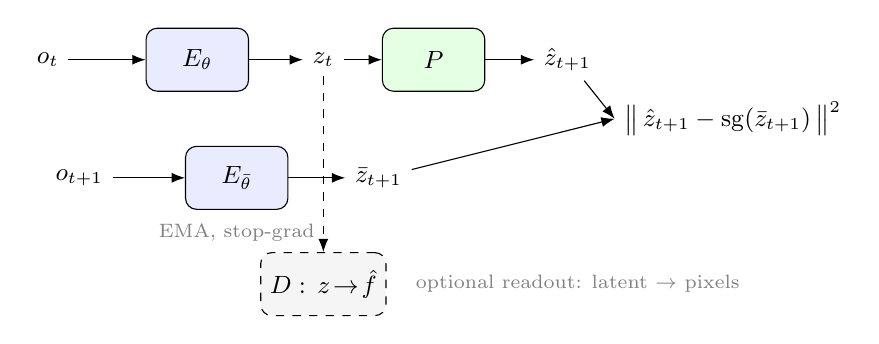
\begin{tikzpicture}[font=\small,>=Latex,
  box/.style={draw,rounded corners,minimum height=8mm,minimum width=13mm,align=center},
  enc/.style={box,fill=blue!8}, pred/.style={box,fill=green!10}, dec/.style={box,fill=gray!8,dashed}]
% online (context) path
\node (ot)   at (0,0)        {$o_t$};
\node[enc] (E1) at (1.9,0)   {$E_\theta$};
\node (zt)   at (3.5,0)      {$z_t$};
\node[pred] (P) at (4.9,0)   {$P$};
\node (zh)   at (6.6,0)      {$\hat z_{t+1}$};
\node (loss) at (8.7,-0.75)  {$\big\lVert\,\hat z_{t+1}-\mathrm{sg}(\bar z_{t+1})\,\big\rVert^{2}$};
% target (EMA, stop-grad) path
\node (ot1)  at (0.4,-1.5)   {$o_{t+1}$};
\node[enc] (E2) at (2.4,-1.5) {$E_{\bar\theta}$};
\node (zb)   at (4.2,-1.5)   {$\bar z_{t+1}$};
\node[font=\scriptsize,gray] at (2.4,-2.2) {EMA, stop-grad};
% optional decoder readout, on its own row
\node[dec] (D) at (3.5,-2.85) {$D:\,z\!\to\!\hat f$};
\node[font=\scriptsize,gray,anchor=west] at (4.55,-2.85) {optional readout: latent $\to$ pixels};
% arrows
\draw[->] (ot)--(E1); \draw[->] (E1)--(zt); \draw[->] (zt)--(P); \draw[->] (P)--(zh);
\draw[->] (zh) -- (loss.west);
\draw[->] (ot1)--(E2); \draw[->] (E2)--(zb);
\draw[->] (zb) -- (loss.west);
\draw[->,dashed] (zt) -- (D);
\end{tikzpicture}
\caption{DVD-JEPA. The predictor matches the EMA target encoder's embedding of the next observation,
entirely in latent space ($\mathrm{sg}$ is stop-gradient). The decoder is an optional readout used only
to visualize and to compute a pixel-space anomaly score.}
\label{fig:arch}
\end{figure}

\paragraph{Objective.} With observations $o_t$ and $o_{t+1}$, we minimize the latent prediction error
plus a VICReg variance term over a batch of online embeddings $Z$:
\begin{equation}
\mathcal{L} \;=\; \big\lVert\, P\!\big(E_\theta(o_t)\big) - \mathrm{sg}\big(E_{\bar\theta}(o_{t+1})\big)\big\rVert^2
\;+\; \sum_{d=1}^{32}\max\!\big(0,\,1-\sigma(Z_{\cdot,d})\big),
\end{equation}
where $\sigma(\cdot)$ is the per-dimension standard deviation and $\mathrm{sg}$ is stop-gradient. The
target encoder is updated as $\bar\theta \leftarrow \tau\bar\theta + (1-\tau)\theta$ with $\tau=0.99$. The
decoder, when used, is trained \emph{separately} on the frozen encoder, so the JEPA performs all of the
representation learning.

\section{Experiments}
\label{sec:exp}
All results use a fixed seed and run on a CPU in ${\sim}10$ seconds for the core model; figures are
regenerated by \texttt{paper/figures.py}.

\paragraph{The representation encodes world state.}
We freeze the encoder and fit a \emph{linear} map from the $32$-d latent to the true $(y,x)$ position.
It achieves \ProbeRMSE\,px RMSE on held-out data in a $16$\,px box---the latent encodes the exact state
of the world despite the model never being shown a coordinate or a reconstruction target.

\paragraph{The stop-gradient prevents collapse.}
Figure~\ref{fig:collapse} tracks the mean embedding standard deviation during training for three
variants. Removing the stop-gradient (making the target trainable) collapses the representation to a
constant ($\sigma\!\to\!0$). The EMA target alone keeps the representation healthy; the variance term is a
safety margin that pins the scale.

\paragraph{The latent rollout forecasts, then drifts.}
We seed from two frames and roll the predictor forward in latent space, decoding each step.
Figure~\ref{fig:horizon} compares the decoded rollout against a persistence baseline (hold the last
observed frame). The model is far more accurate for the near horizon and degrades gracefully; the
filmstrip (Figure~\ref{fig:film}) shows it correctly imagining the bounce for ${\sim}20$ steps before
single-step errors compound. Mean prediction MSE rises from \ForecastStepOne{} at one step to
\ForecastStepK{} at \ForecastHorizon{} steps.

\paragraph{Prediction error is a usable anomaly signal.}
Run as a one-step monitor, the model renders what it expects next; when reality diverges, the pixel error
spikes. We inject a teleport at frame~\AnomalyInjected{}; the surprise peaks \AnomalyPeak$\times$ over
baseline and is flagged at frame~\AnomalyDetected{} (Figure~\ref{fig:anomaly}), two frames early because
the monitor predicts two steps ahead.

\begin{figure}[t]
\centering
\begin{subfigure}{0.49\textwidth}\centering
  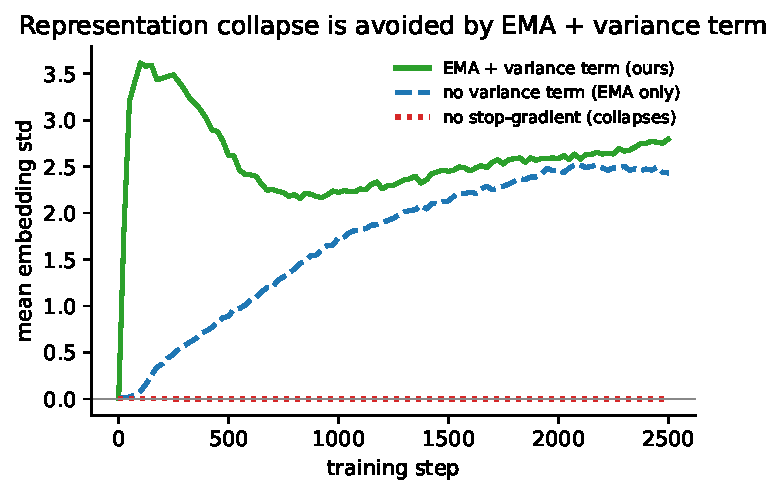
\includegraphics[width=\linewidth]{fig/fig_collapse.pdf}
  \caption{Anti-collapse ablation.}\label{fig:collapse}
\end{subfigure}\hfill
\begin{subfigure}{0.49\textwidth}\centering
  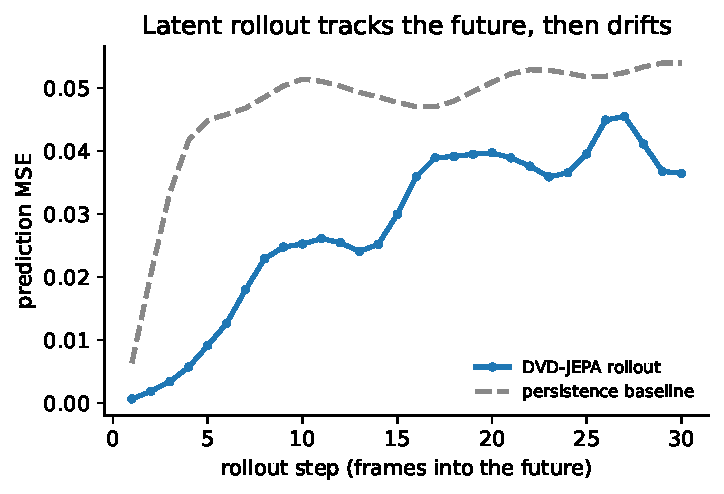
\includegraphics[width=\linewidth]{fig/fig_horizon.pdf}
  \caption{Forecast horizon vs.\ a persistence baseline.}\label{fig:horizon}
\end{subfigure}
\caption{Left: removing the stop-gradient collapses the representation; the EMA target prevents it.
Right: the latent rollout tracks the future far better than persistence, then drifts as errors compound.}
\end{figure}

\begin{figure}[t]
\centering
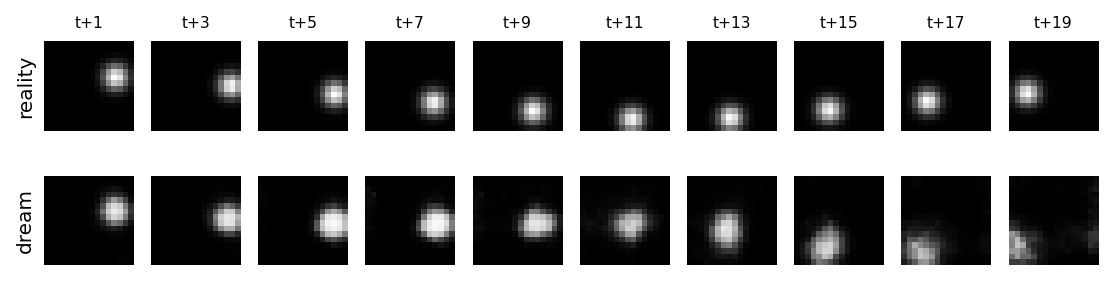
\includegraphics[width=0.92\textwidth]{fig/fig_filmstrip.png}
\caption{Future-frame prediction. Top: reality. Bottom: the decoded latent dream, rolled forward in
representation space. It reproduces the trajectory and the wall bounce for roughly twenty steps.}
\label{fig:film}
\end{figure}

\begin{figure}[t]
\centering
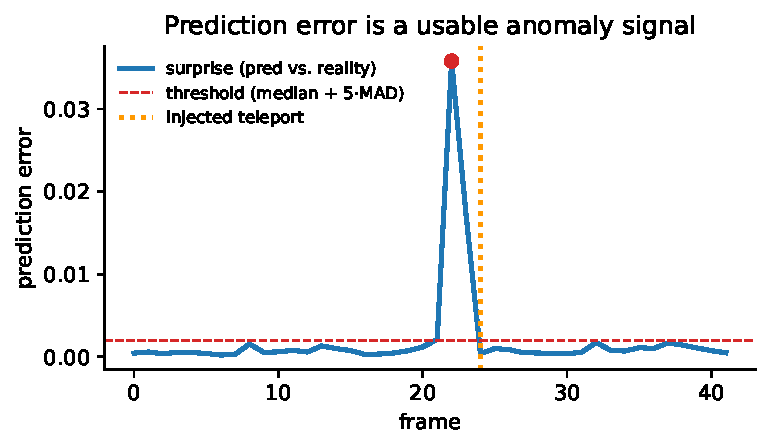
\includegraphics[width=0.66\textwidth]{fig/fig_anomaly.pdf}
\caption{DVD-JEPA as a predictive anomaly detector. A teleport injected at frame \AnomalyInjected{}
produces a surprise spike \AnomalyPeak$\times$ over baseline, crossing the threshold.}
\label{fig:anomaly}
\end{figure}

\section{Interactive Demo}
The trained networks are exported as base64 float32 and re-implemented in dependency-free JavaScript, so
the model runs entirely client-side at \href{https://dvd-jepa.vercel.app}{\texttt{dvd-jepa.vercel.app}}
(no server, no GPU). A viewer can toggle the decoder off to see that a \emph{pure} JEPA returns only a
$32$-vector and cannot draw; inject anomalies and watch the surprise meter; and roll the predictor forward
to watch multi-step latent drift. We find that manipulating the model in real time conveys the
predict-in-representation-space idea more directly than static figures.

\section{Related Work}
DVD-JEPA is a miniature of I-JEPA~\cite{assran2023} and V-JEPA~\cite{bardes2024}, which apply the same
predict-in-latent-space objective with EMA target encoders at Vision-Transformer scale, and of
V-JEPA~2~\cite{vjepa2}, which adds action-conditioning for planning. The anti-collapse machinery follows
BYOL~\cite{grill2020} and VICReg~\cite{bardes2022}. It contrasts with \emph{generative} world models
such as World Models~\cite{ha2018} and Dreamer~\cite{hafner2020}, which predict in pixel or reconstructed
latent space and can render but must model irreducible detail. DVD-JEPA is, deliberately, the non-generative
counterpart shrunk to a size one can hold in one's head.

\section{Limitations}
The world is $16\times16$ and deterministic, so there is no need for a stochastic latent to model
multi-modal futures (real JEPAs include one). The predictor is trained for a single step, so autoregressive
rollouts drift after ${\sim}20$ steps; multi-step or recurrent training would extend the horizon. The
decoder is a crutch added only for visualization and pixel-space scoring---a pure JEPA has none. Finally,
the demonstrations are qualitative-scale: the value of DVD-JEPA is pedagogical transparency, not a new
state of the art.

\section{Conclusion}
DVD-JEPA shows that a complete, correct JEPA world model---representation-space prediction, EMA target,
anti-collapse, latent rollout, and an optional rendering head---fits in a few hundred lines and trains on
a CPU in seconds. It learns the physics of a bouncing logo with no labels, forecasts the future, and
detects anomalies, while remaining small enough to inspect end to end and interactive enough to play with
in a browser. We hope it serves as a runnable on-ramp to the full-scale systems it imitates.

\paragraph{Reproducibility.} Code, trained weights, the interactive demo, and a Colab notebook are at
\href{https://github.com/mandarwagh9/dvd-jepa}{\texttt{github.com/mandarwagh9/dvd-jepa}}. Running
\texttt{python -m dvd\_jepa.train} reproduces the model and \texttt{python paper/figures.py} reproduces
every figure and number in this paper.

\begin{thebibliography}{9}
\small
\bibitem{lecun2022} Y.~LeCun. \emph{A Path Towards Autonomous Machine Intelligence}. Open Review, 2022.
\bibitem{assran2023} M.~Assran et al. \emph{Self-Supervised Learning from Images with a Joint-Embedding
Predictive Architecture (I-JEPA)}. CVPR, 2023.
\bibitem{bardes2024} A.~Bardes et al. \emph{Revisiting Feature Prediction for Learning Visual
Representations from Video (V-JEPA)}. TMLR, 2024.
\bibitem{vjepa2} Meta AI. \emph{V-JEPA~2: Self-Supervised Video Models Enable Understanding, Prediction
and Planning}. 2025.
\bibitem{bardes2022} A.~Bardes, J.~Ponce, Y.~LeCun. \emph{VICReg: Variance-Invariance-Covariance
Regularization for Self-Supervised Learning}. ICLR, 2022.
\bibitem{grill2020} J.-B.~Grill et al. \emph{Bootstrap Your Own Latent (BYOL)}. NeurIPS, 2020.
\bibitem{ha2018} D.~Ha, J.~Schmidhuber. \emph{World Models}. NeurIPS, 2018.
\bibitem{hafner2020} D.~Hafner et al. \emph{Dream to Control: Learning Behaviors by Latent Imagination
(Dreamer)}. ICLR, 2020.
\end{thebibliography}

\end{document}
